\documentclass[handout]{ximera}
%handout:  for handout version with no solutions or instructor notes
%handout,instructornotes:  for instructor version with just problems and notes, no solutions
%noinstructornotes:  shows only problem and solutions

%% handout
%% space
%% newpage
%% numbers
%% nooutcomes

%I added the commands here so that I would't have to keep looking them up
%\newcommand{\RR}{\mathbb R}
%\renewcommand{\d}{\,d}
%\newcommand{\dd}[2][]{\frac{d #1}{d #2}}
%\renewcommand{\l}{\ell}
%\newcommand{\ddx}{\frac{d}{dx}}
%\everymath{\displaystyle}
%\newcommand{\dfn}{\textbf}
%\newcommand{\eval}[1]{\bigg[ #1 \bigg]}

%\begin{image}
%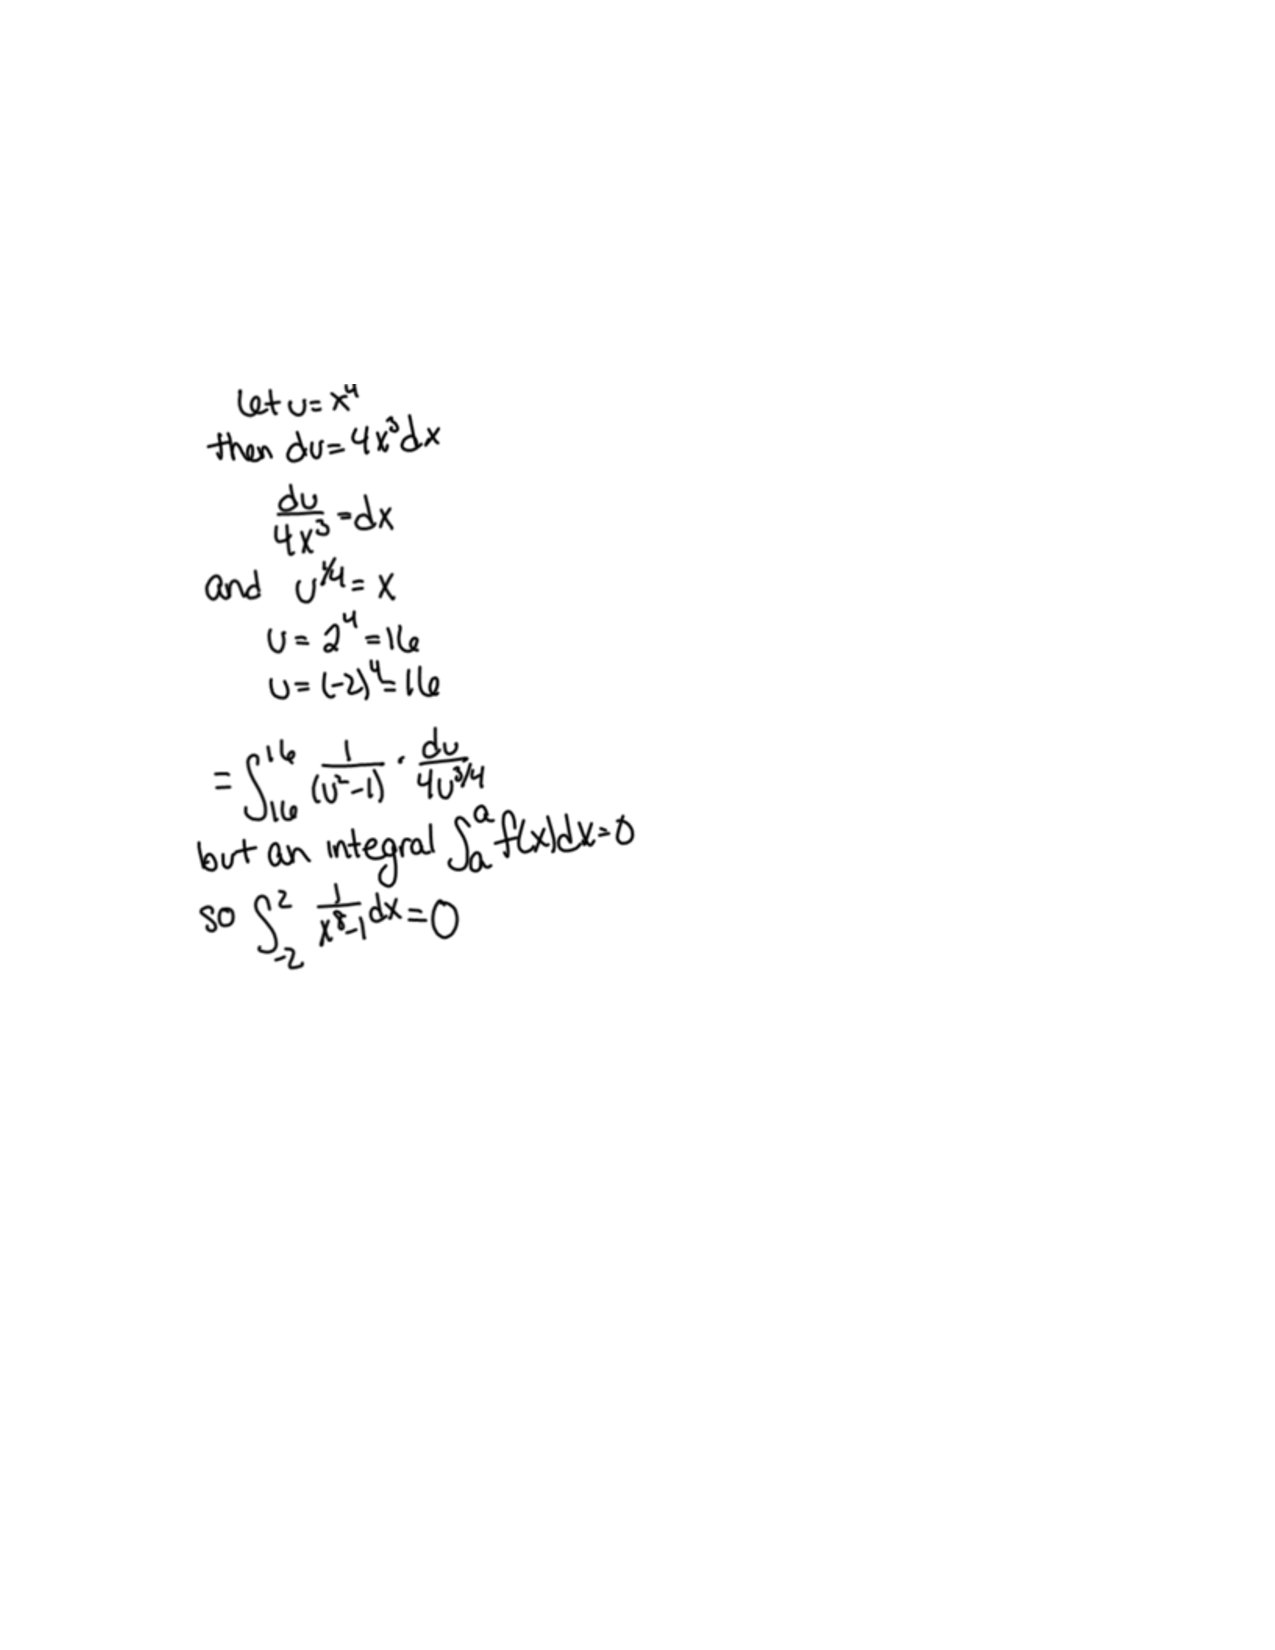
\includegraphics[trim= 170 420 250 180]{Figure1.pdf}
%\end{image}

%add a ``.'' below when used in a specific directory.
\newcommand{\RR}{\mathbb R}
\renewcommand{\d}{\,d}
\newcommand{\dd}[2][]{\frac{d #1}{d #2}}
\renewcommand{\l}{\ell}
\newcommand{\ddx}{\frac{d}{dx}}
\newcommand{\dfn}{\textbf}
\newcommand{\eval}[1]{\bigg[ #1 \bigg]}

\usepackage{multicol}

\renewenvironment{freeResponse}{
\ifhandout\setbox0\vbox\bgroup\else
\begin{trivlist}\item[\hskip \labelsep\bfseries Solution:\hspace{2ex}]
\fi}
{\ifhandout\egroup\else
\end{trivlist}
\fi} %% we can turn off input when making a master document

\title{Direction fields and Euler's method}  

\begin{document}
\begin{abstract}		\end{abstract}
\maketitle



\begin{comment}
\section{Warm up:}

	\begin{freeResponse}
	
	\end{freeResponse}
	
\begin{instructorNotes}

\end{instructorNotes}
\end{comment}







\section{Group work:}



%problem 1
\begin{problem}
	
	\begin{enumerate}
	\item  The following is a direction field for the differential equation $\dd[y]{x} = y^2 - x^2$.
	
		\begin{image}
		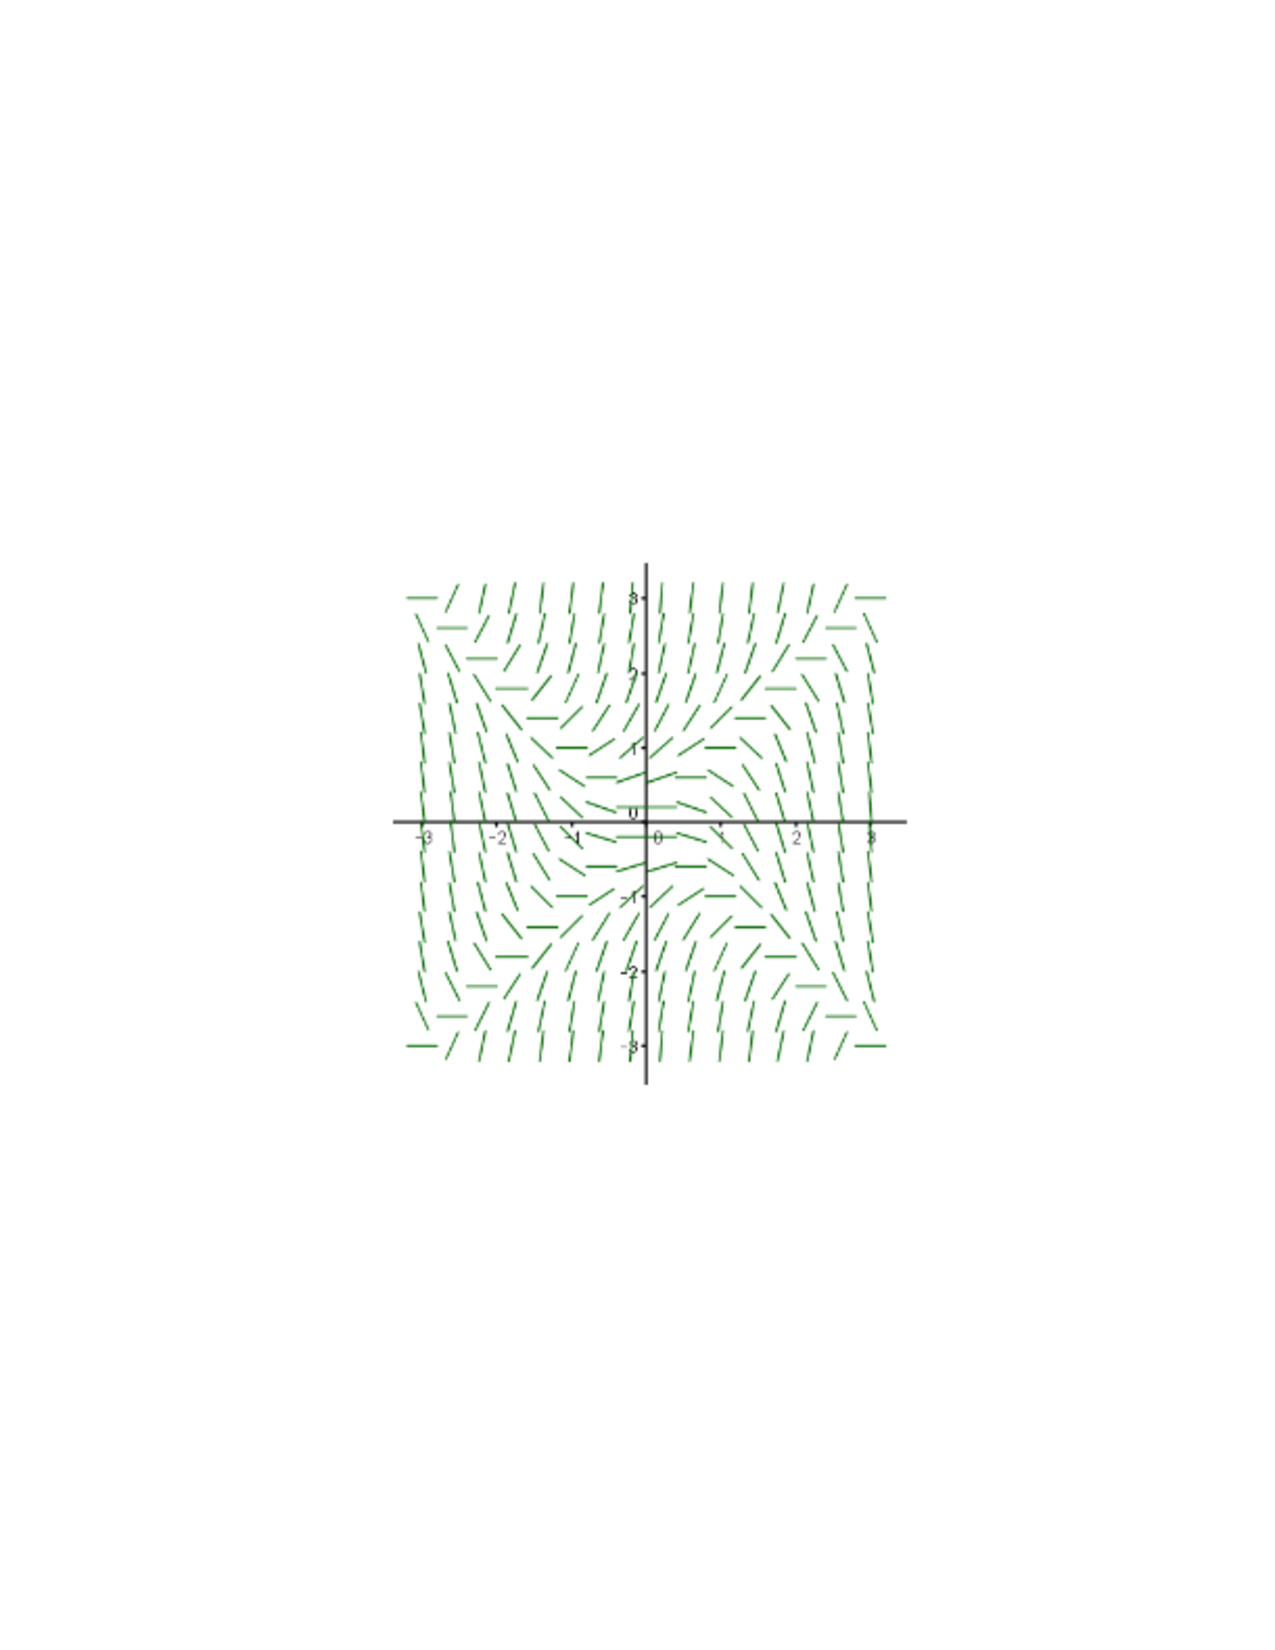
\includegraphics[trim= 300 280 250 280,scale=0.8]{Figure8-2-1.pdf}
		\end{image}
		
		Sketch the solution such that $y\left( \frac{1}{2} \right) = 1$.
	\begin{freeResponse}
	
	\begin{image}
	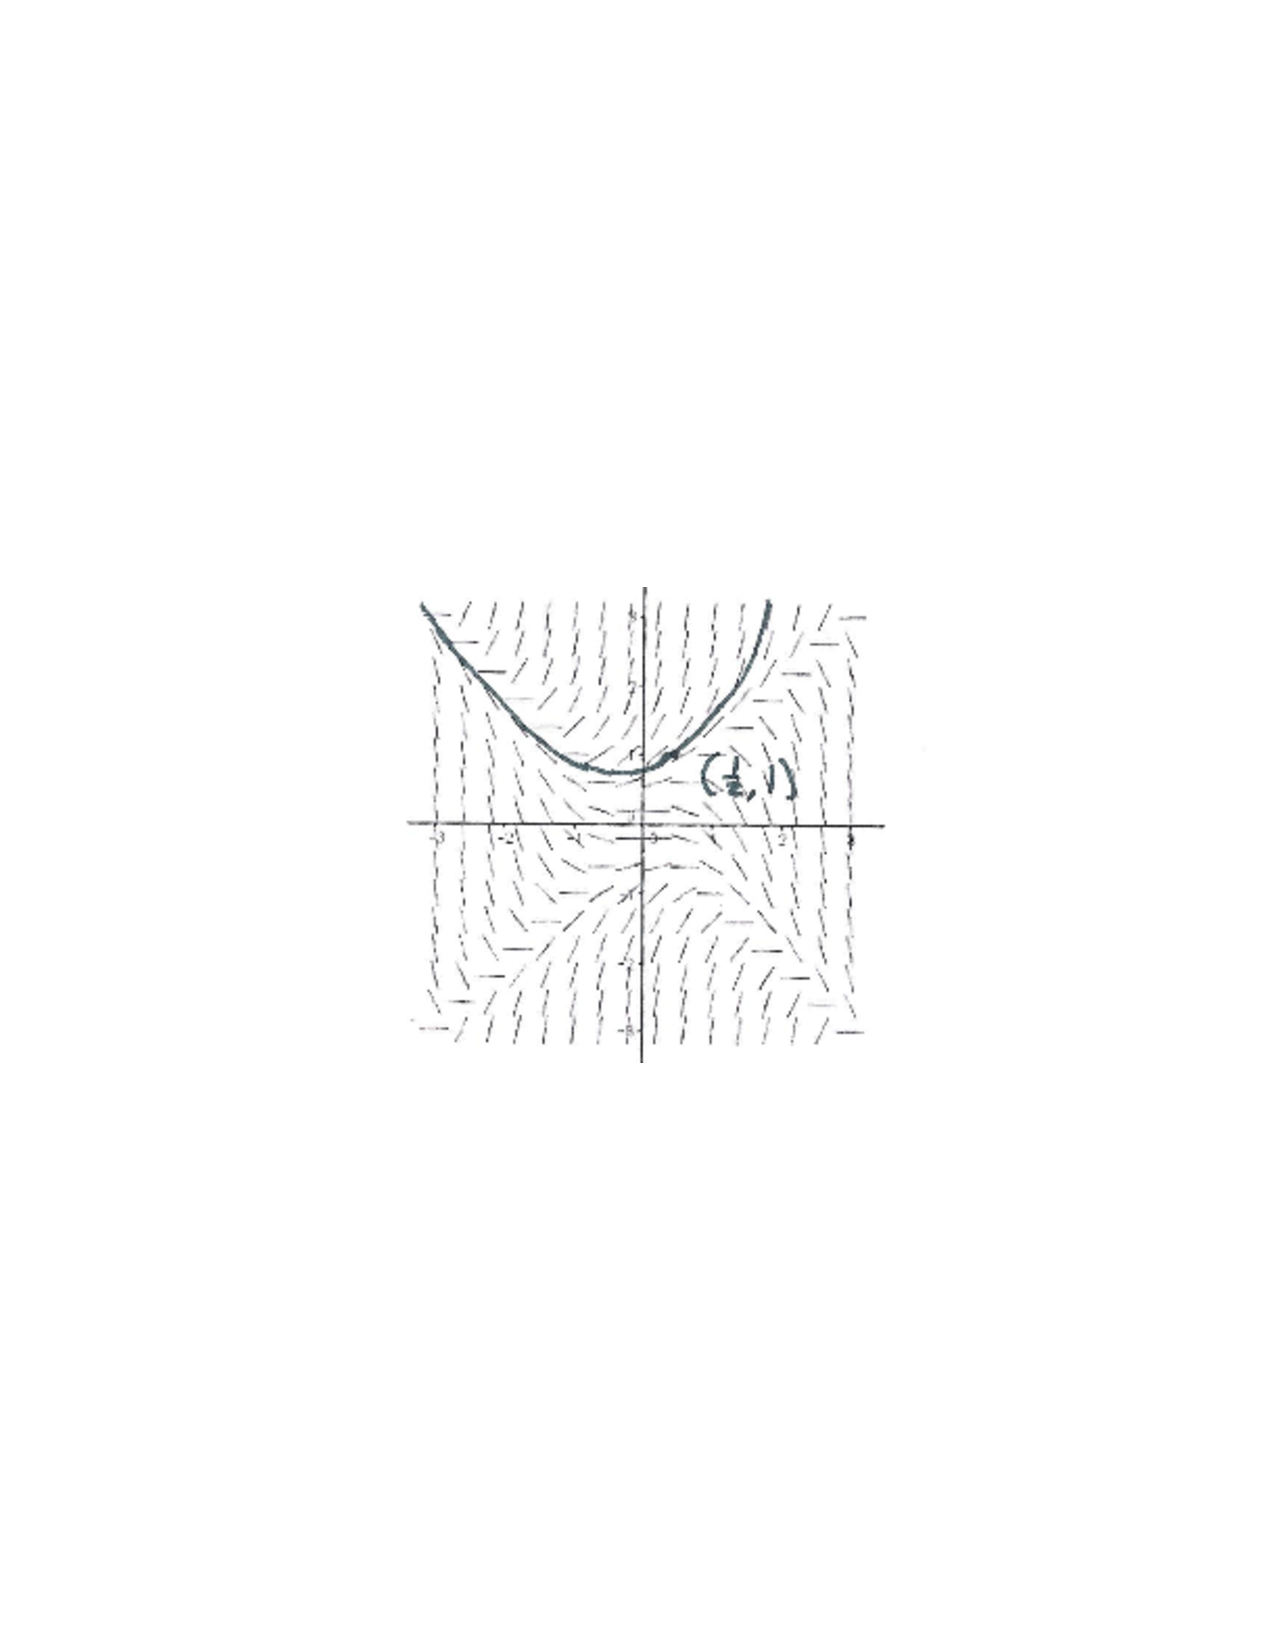
\includegraphics[trim= 330 260 250 300,scale=0.8]{Figure8-2-4.pdf}
	\end{image}
	
	\end{freeResponse}
	
	
	
	\item  Use Euler's Method to give a numerical estimate to the solution of the differential equation $y' = y^2 - t^2$ at $y(2)$ that goes through the point $\left( \frac{1}{2}, 1 \right)$.  
	Use $\Delta t = 0.5$.
	\begin{freeResponse}
	
		%\begin{table}[]
		%\centering
		\begin{tabular}{|c|c|c|c|}
		\hline
		 $T$ 	& 	$y$ 	 & 	$\dd[y]{t}=y^2-t^2$ 	 &	$y + \dd[y]{t} \cdot \Delta t$   	\\
		 \hline
		 $0.5$	&	$1$	  &	$0.75$		  	&	$1.375$	\\
		 \hline
		 $1$	&	$1.375$  &	$0.890625$		  	&	$1.820313$   \\
		 \hline
		 $1.5$	&	$1.820313$  &	$1.063538$		&	$2.352081$    \\
		 \hline
		 $2$	&	$2.352081$  &  &    \\
		 \hline
		\end{tabular}
		%\end{table}
		
	So, $y(2) \approx 2.352081$.
	\end{freeResponse}
	\end{enumerate}
	
\end{problem}

\begin{instructorNotes}
The major point here is that (a) and (b) are the same problem, presented with two different representations.
\end{instructorNotes}







%problem 2
\begin{problem}
Describe why the following direction field could be the direction field for the differential equation 
	\[
	\dd[y]{t} y \cos(t)
	\]
but \dfn{not} for 
	\[
	\dd[y]{t} = y \sin(t) 	\qquad	\text{or}	\qquad	\dd[y]{t} = t \cos(y).
	\]
	
	\begin{image}
	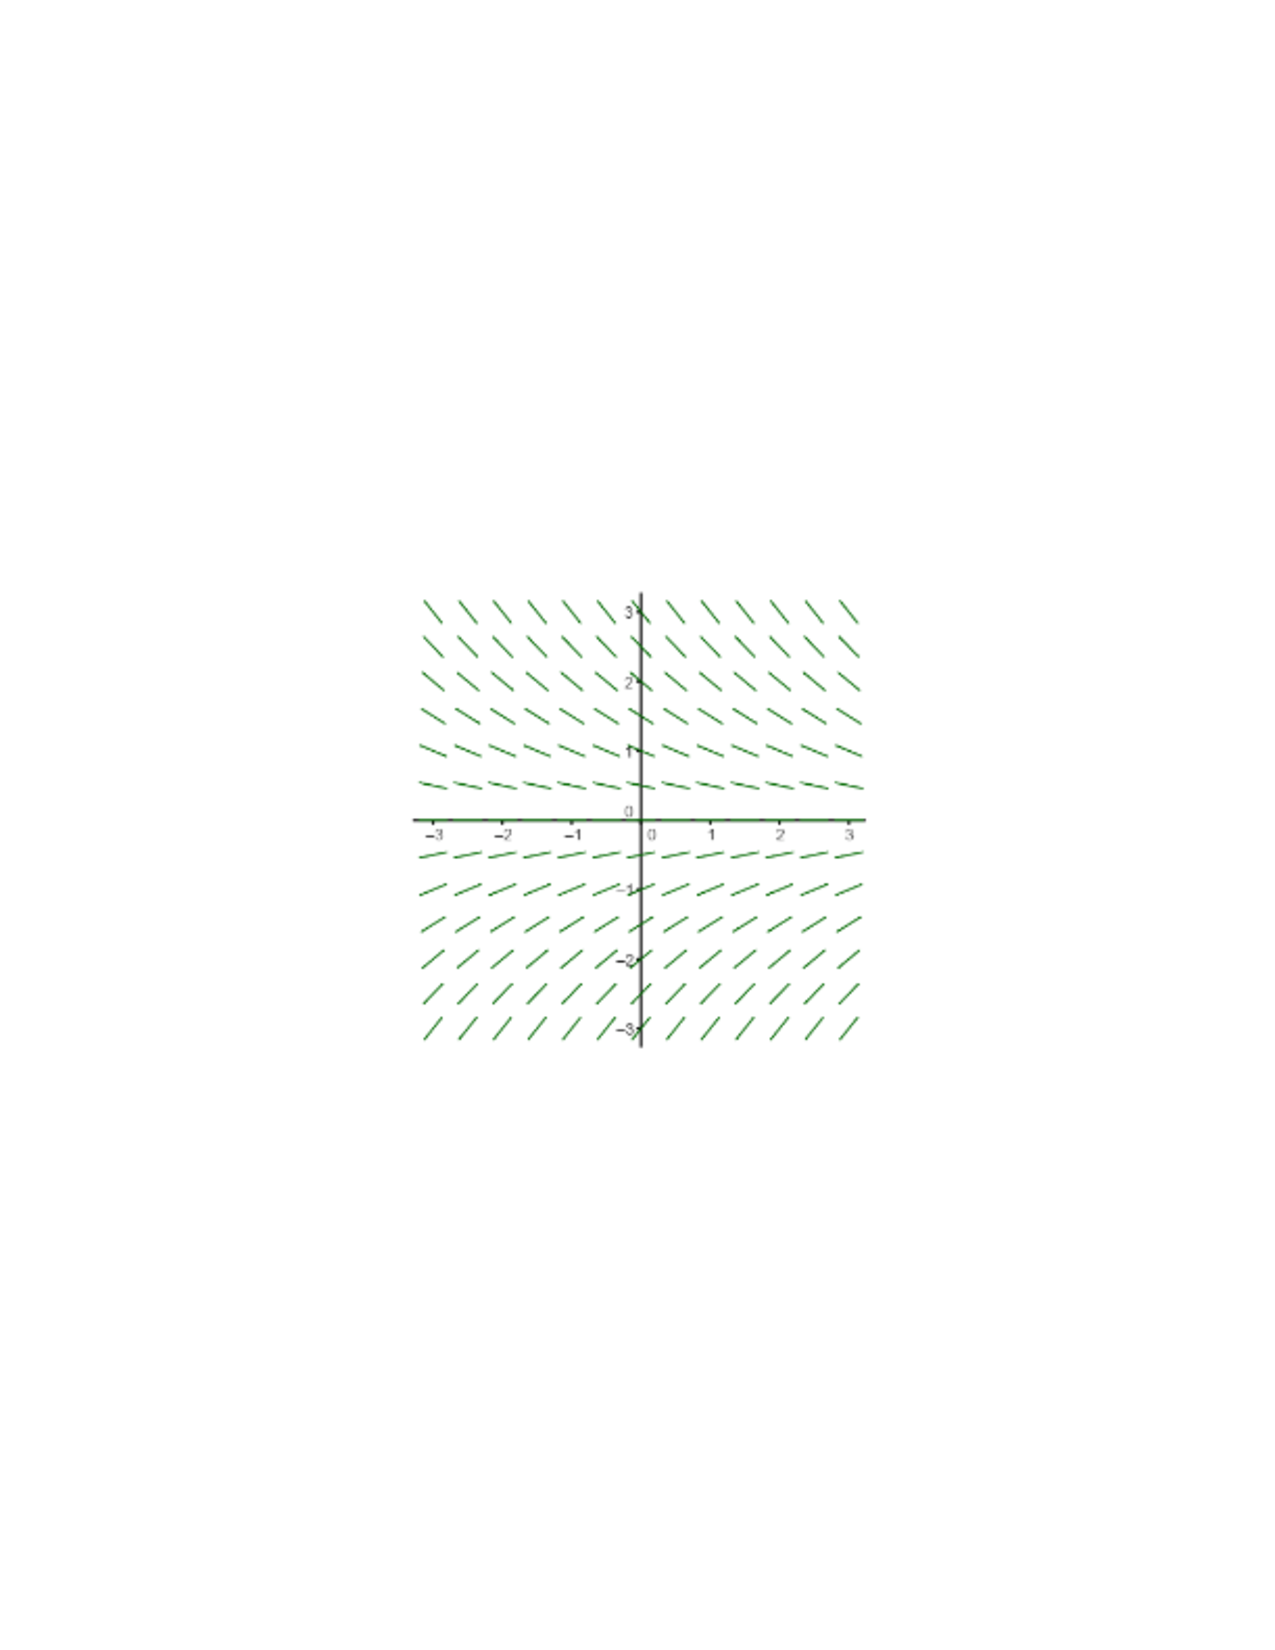
\includegraphics[trim= 300 280 250 280,scale=0.8]{Figure8-2-2.pdf}
	\end{image}
	\begin{freeResponse}
		
	Look along the line $t=0$ (the $y$-axis).
	
	\begin{itemize}
	
	\item  For $\dd[y]{t} = y \sin(t)$:
	
	$\eval{\dd[y]{t}}_{t=0} = y \sin(0) = 0$.  
	But this direction field does not have horizontal tangents at each point along $t=0$.  
	So it \dfn{cannot} be the direction field for $\dd[y]{t} = y \sin(t)$.
	
	\item  For $\dd[y]{t} = t \cos(y)$:
	
	$\eval{\dd[y]{t}}_{t=0} = (0) \cos(y) = 0$.  
	But again this direction field does not have horizontal tangents at each point along $t=0$.  
	So it \dfn{cannot} be the direction field for $\dd[y]{t} = t \cos(y)$.
	
	\item  For $\dd[y]{t} y \cos(t)$:
	
	Along $t=0$, this equation is $\dd[y]{t} = y \cos(0) = y$.  
	However, when $y$ is positive, the slopes are negative.  
	Also, when $y$ is negative, the slopes are positive.  
	So this is \dfn{not} the direction field for $\dd[y]{t} = y \cos(t)$, either.
	
	\end{itemize}
	\end{freeResponse}
		
\end{problem}

\begin{instructorNotes}
Students should examine when $t$ varies across quadrants, combined with the sign of $y$ at points $(t,y)$ (with $y'=t \cos y$, $y$ is going through ``quadrants'').  Checking where $y'=0$ can reveal why the other two differential equations are not satisfied.  
This could all just be a whole class discussion with the instructor bringing up strategies.
\end{instructorNotes}







%problem 3
\begin{problem}
Match each of the following differential equations with a corresponding direction field (if it is present):
	\begin{multicols}{2}
	\begin{enumerate}
	\item[i.]	$y' = \frac{t}{2+y}$
	\item[ii.]	$y' = \cos(t+y)$
	\item[iii.]	$y' = 1+y^2$
	\item[iv.]	$y' = ty$
	\end{enumerate}
	\end{multicols}
	
	\begin{image}
	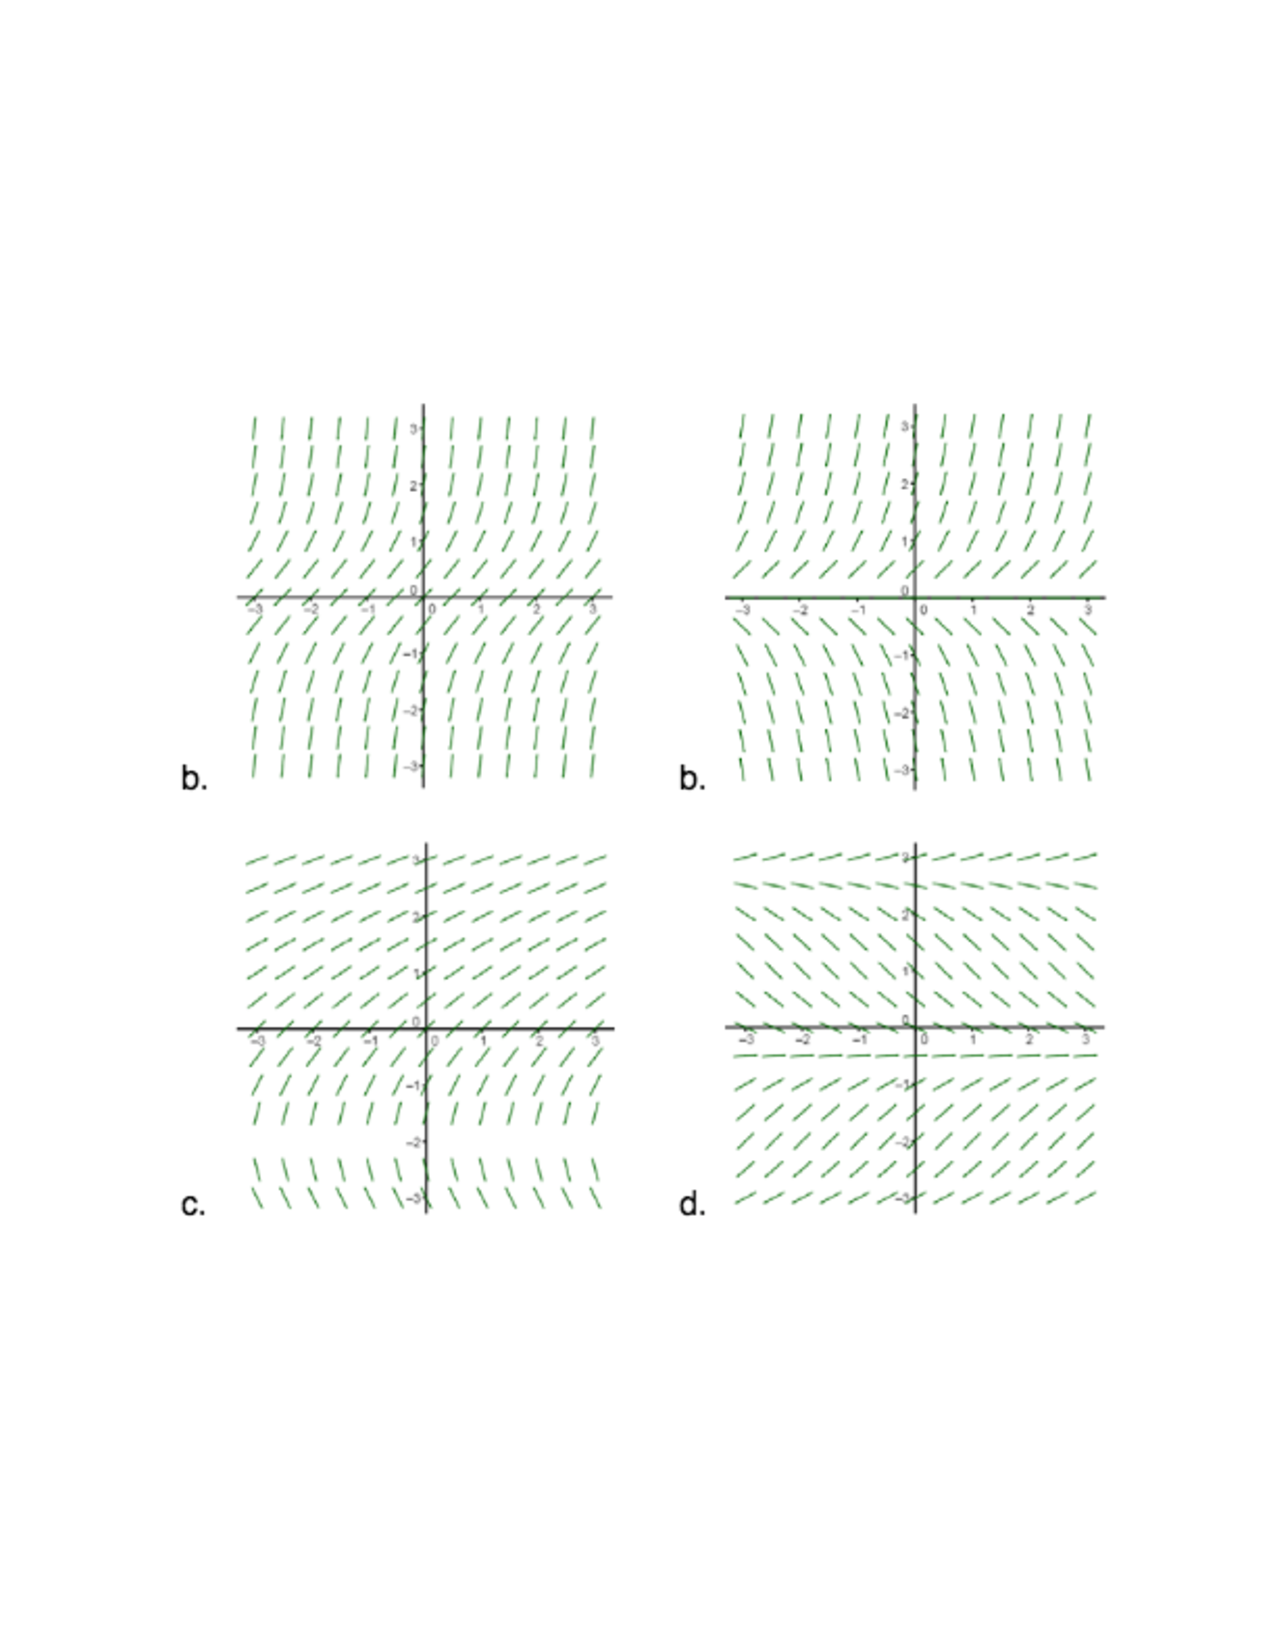
\includegraphics[trim= 250 200 250 200,scale=0.8]{Figure8-2-3.pdf}
	\end{image}
	
	\begin{freeResponse}
	Look along the line $t=0$ (the $y$-axis).
	\begin{enumerate}
	
	\item[(i)] $y' = \frac{t}{2+y}$ and (iv) $y'=ty$ must both be identically $0$ along the $y$-axis.  
	However, none of the direction fields given have horizontal slopes along the $y$-axis.  
	So none of them can be the direction field for (i) or (iv).  
	
	\item[(ii)]  At the origin, we have $y' = \cos(t+y) = \cos(0) = 1$.  
	So the direction field for (ii) must have slope $1$ at the origin.  
	This eliminates (b) and (d).  
	Now look at the point $\left( 0, \frac{\pi}{2} \right)$.  
	We have $\eval{y'}_{(0,\frac{\pi}{2})} = \cos \left( \frac{\pi}{2} \right) = 0$, so the direction field must be horizontal at that point.  
	That means that it cannot be (a) or (c) either.
	
	\item[(iii)]  Here $y' = 1+y^2$, so there is no $t$ on the right hand side of the equation.  
	Therefore, $y'$ depends only on $y$.  
	At $y=0$ the slope is $1$, then as $y$ increases the slopes increase too.  
	Similarly, as $y$ gets more and more negative, the slope gets more and more positive.  
	So it seems as if this direction field is (a).
	
	\end{enumerate}
	\end{freeResponse}

\end{problem}

\begin{instructorNotes}
Several strategies exist.  
Make sure to ask what special quality direction fields of autonomous differential equations have.  
Depending on time, this also could all be done as a whole class.
\end{instructorNotes}






%Problem 4
\begin{problem}
Which of the following are separable differential equations?
For those that are, solve them, assuming that $y(4)=5$.
	\begin{enumerate}
	\item 	$y' = x^2+y^2$
	\begin{freeResponse}
	This differential equation is \dfn{not} separable.
	\end{freeResponse}
	
	
	
	\item 	$y'=x+xy^2$
	\begin{freeResponse}
		\begin{align*}
		&y' = x+xy^2  \\
		\Longrightarrow 	\qquad	&\dd[y]{x} = x(1+y^2)  \\
		\Longrightarrow 	\qquad	&\frac{\d y}{1+y^2} = x \d x.
		\end{align*}
	So this equation \dfn{is} separable.
	To solve, we integrate both sides of the equation:
		\begin{align}
		&\int \frac{1}{1+y^2} \d y = \int x \d x  \nonumber \\
		\Longrightarrow 	\qquad	&\arctan(y) = \frac{1}{2} x^2 + C  \label{equation 1 for y}\\
		\Longrightarrow 	\qquad	&y = \tan \left( \frac{1}{2} x^2 + C \right).  \nonumber
		\end{align}
	To find $C$, we plug the initial condition $y(4) = 5$ into equation \eqref{equation 1 for y} and solve for $C$.
		\begin{align*}
		&\arctan(5) = \frac{1}{2} (4)^2 + C = 8 + C  \\
		\Longrightarrow 	\qquad	&C = \arctan(5) - 8.
		\end{align*}
	So
		\[
		y = \tan \left( \frac{1}{2} x^2 + \arctan(5) - 8 \right).
		\]
	\end{freeResponse}
	
	
	
	\item 	$y' = e^{2x-y}$
	\begin{freeResponse}
		\begin{align}
		&y' = e^{2x-y}  \nonumber \\
		\Longrightarrow 	\qquad	&\dd[y]{x} = \frac{e^{2x}}{e^y}  \nonumber \\
		\Longrightarrow 	\qquad	&e^y \d y = e^{2x} \d x  \label{eqn 2}
		\end{align}
	and so this \dfn{is} a separable equation.  
	To solve, we integrate both sides of equation \eqref{eqn 2}.
		\begin{align}
		&\int e^y \d y = \int e^{2x} \d x  \nonumber  \\
		\Longrightarrow 	\qquad	&e^y = \frac{1}{2} e^{2x} + C  \label{eqn 3}  \\
		\Longrightarrow 	\qquad	&y = \ln \left( \frac{1}{2} e^{2x} + C \right).  \nonumber
		\end{align}
	To find $C$, we plug into equation \eqref{eqn 3} and solve for $C$:
		\begin{align*}
		&e^5 = \frac{1}{2} e^8 + C  \\
		\Longrightarrow 	\qquad	&C = e^5 - \frac{1}{2} e^8.
		\end{align*}
	Therefore
		\[
		y = \ln \left( \frac{1}{2} e^{2x} + e^5 - \frac{1}{2}e^8 \right).
		\]
	\end{freeResponse}
	\end{enumerate}
	
\end{problem}

\begin{instructorNotes}
Part (b) is the only non-separable equation.  
Students may need help recognizing that they can divide by the entire right side of both sides.  
Also, some results may only define $y$ implicitly.
\end{instructorNotes}










	
	
	
	
	
	
	
	
	

	










								
				
				
	














\end{document} 


















